%% Knowledge-Based Systems / Elsevier CAS manuscript package.
%% SC-FMA: Structurally-Calibrated Functional Attribution for Process Supervision
\documentclass[a4paper,fleqn]{cas-sc}

\usepackage[numbers,sort&compress]{natbib}
\usepackage{amsmath}
\usepackage{booktabs}
\usepackage{array}
\usepackage{graphicx}
\usepackage{xurl}
\usepackage{amsthm}
\newtheorem{theorem}{Theorem}[section]
\newtheorem{lemma}[theorem]{Lemma}
\newtheorem{corollary}[theorem]{Corollary}
\usepackage{algorithm}
\usepackage{algpseudocode}
\usepackage{multirow}
\usepackage{makecell}
\usepackage{placeins}
\usepackage{CJKutf8}
\usepackage{xr}
\usepackage{hyperref}
\hypersetup{colorlinks=true,linkcolor=blue,citecolor=blue,urlcolor=blue}
\externaldocument[][nocite]{supplementary}
\newcolumntype{Z}[1]{>{\raggedright\arraybackslash}p{#1}}
\newcommand{\wstruct}{\ensuremath{\mathbf{w}_{\mathrm{struct}}}}

\begin{document}
\let\WriteBookmarks\relax
\def\floatpagepagefraction{1}
\def\textpagefraction{.001}
\pagenumbering{arabic}

\shorttitle{Structurally-Calibrated Functional Attribution}
\shortauthors{Ma and Wang}

\title[mode=title]{Structurally-Calibrated Functional Attribution for Audit Prioritization in Knowledge-Intensive Reasoning}

\author[1]{Haoran Ma}
\ead{mahaoran0000@foxmail.com}

\author[1,2]{Ningning Wang\corref{cor1}}
\ead{wangningning@bistu.edu.cn}

\cortext[cor1]{Corresponding author.}
\renewcommand{\printorcid}{}

\affiliation[1]{organization={College of Management Science and Engineering, Beijing Information Science and Technology University},
            city={Beijing},
            postcode={102200},
            country={China}}

\affiliation[2]{organization={Institute of Information Systems, ESG Intelligent Application Innovation Research Center},
            city={Beijing},
            postcode={102200},
            country={China}}

\begin{abstract}
Knowledge-intensive reasoning systems expose intermediate traces, yet fixed-budget review still lacks a principled way to decide which steps to inspect and what audit action each step requires. Scalar process scores rank steps but collapse distinct roles such as local evidential support, redundant checks, and downstream bottlenecks. We introduce Structurally-Calibrated Functional Attribution (SC-FMA), which converts a supplied utility or proxy-fidelity signal and an observable reasoning trace into a graph-aware audit queue. The Structurally-Calibrated Utility (SCU) objective solves a convex step-weighting problem that preserves informative fidelity while adding necessity, redundancy, and bottleneck diagnostics. We evaluate SC-FMA through an Evidence Ladder comprising controlled synthetic calibration, a Countries-KG typed-edge stage, PRM800K process-supervision annotations (4,417 samples and 34,219 labeled steps under a frozen hash split), and automatic audit-target validation. On the controlled synthetic stage, SC-FMA QP raises Spearman $\rho$ with proxy step labels from 0.483 to 0.597. On PRM800K, the learned fidelity signal remains the strongest ranker ($\rho=0.611$), while SC-FMA Ridge closely preserves it ($\rho=0.604$; NDCG@25\% 0.946 versus 0.951) and exposes audit fields. The Countries-KG stage shows typed-edge feasibility, with KG augmentation reordering structural necessity (mean absolute delta 0.431). In the automatic audit-target stage, SC-FMA decomposition improves Recall@25\% from 0.235 to 0.699 and NDCG@25\% from 0.353 to 0.978 over a scalar-only view. SC-FMA therefore provides a signal-preserving audit-prioritization layer for observable reasoning traces, bounded to audit triage and local functional attribution.
\end{abstract}

\begin{keywords}
structural calibration \sep functional attribution \sep audit prioritization \sep process supervision \sep knowledge-based systems
\end{keywords}

\maketitle

\section{Introduction}

Knowledge-intensive reasoning systems increasingly expose inspectable traces after prediction. Step-level supervision has shown that intermediate verification can reveal errors hidden by final-answer accuracy~\cite{lightman2023verify,uesato2022solving}. Retrieval-augmented and knowledge-graph-augmented pipelines add retrieved passages~\cite{lewis2020rag} and entity-relation structure~\cite{edge2024graphrag} as review objects. The practical bottleneck is no longer whether traces exist, but which elements deserve attention under a limited audit budget.

A flat salience score can order trace elements, but it rarely tells a reviewer how to act on that order. A high-ranked step may be locally reliable, structurally necessary, redundant with neighboring evidence, or a bottleneck for downstream reasoning. These distinctions matter in KBS settings such as rule chains, retrieval-augmented workflows, and KG-assisted reasoning, where inspection time is limited and different structural roles imply different audit actions.

This paper studies audit prioritization as intervention-based functional attribution over observable reasoning traces. We propose Structurally-Calibrated Functional Attribution (SC-FMA), a structural calibration layer that preserves an informative utility or proxy-fidelity signal while adding graph necessity, redundancy, and bottleneck diagnostics. The Structurally-Calibrated Utility (SCU) objective implements this calibration as a convex weighting problem over process steps, producing both a rank and an audit record.

The main findings are summarized as follows:

\begin{itemize}
  \item On the controlled synthetic stage, SC-FMA QP exhibits the intended calibration behavior in a high-structure-conflict setting, increasing mean Spearman correlation with proxy step labels from $0.483$ for raw CIU to $0.597$. A component ablation shows that the fidelity signal is the essential signal, while redundancy and bottleneck terms act as conditional regularizers whose contribution scales with structural preference in the labels.
  \item On PRM800K process-supervision annotations (4,417 samples and 34,219 labeled steps under a frozen hash split), \wstruct{} is the primary direct ranker (Spearman $\rho = 0.611$). SC-FMA Ridge closely preserves it ($\rho = 0.604$) while exposing decomposition fields for audit.
  \item An automatic audit-target validation provides rule-derived (non-human) evidence that SC-FMA decomposition retrieves bottleneck, redundancy, weak-anchor, and structural-overcorrection targets more effectively than a scalar-only view. Mean Recall@25\% increases from $0.235$ to $0.699$, and mean NDCG@25\% increases from $0.353$ to $0.978$.
  \item A Sentence-BERT graph-construction ablation and the fixture-level Countries-KG typed-edge stage show that the graph layer can accept a semantic-embedding backend and typed ontology edges at the same interface.
\end{itemize}

The paper makes three contributions. First, it formulates fixed-budget audit of reasoning traces as an audit-prioritization problem. Second, it introduces SC-FMA and the SCU objective, which convert fidelity or utility inputs into structurally calibrated verification-step weights with formal guarantees and decomposition fields. Third, it evaluates the method through an Evidence Ladder that moves from controlled synthetic calibration to Countries-KG typed-edge feasibility, PRM800K step-label ranking, and rule-derived audit-target validation. Section~\ref{sec:claim-boundary} states the evidence boundary and future validation directions.

The remainder of this paper is organized as follows. Section~\ref{sec:related-work} reviews attribution, process supervision, and graph-based KBS audit methods, and identifies the research gap. Section~\ref{sec:methods} presents the SC-FMA method, the SCU objective, and its theoretical properties. Section~\ref{sec:experimental-results} reports the Evidence Ladder. Section~\ref{sec:discussion} interprets the results, and Section~\ref{sec:conclusions} concludes.

Figure~\ref{fig:overall-framework} gives the high-level audit workflow. SC-FMA starts from a scalar fidelity signal and an observable reasoning trace, builds a trace-level audit graph, calibrates the signal against structural diagnostics, and returns a fixed-budget audit queue with an explicit rationale and action for each selected step.

\begin{figure}[pos=ht]
\centering

\includegraphics[width=\linewidth]{figures/fig_overall_framework.pdf}
\caption{Overall SC-FMA audit-prioritization framework. A scalar fidelity signal and an observable reasoning trace are converted into a structure-aware audit representation. The SC-FMA layer builds an audit graph, applies SCU calibration, and carries fidelity, necessity, redundancy, bottleneck, and review-action fields into the audit record. The output is a bounded audit queue with step-specific reasons and actions rather than an uninterpreted scalar ranking.}
\label{fig:overall-framework}
\end{figure}

\section{Related Work}
\label{sec:related-work}

\subsection{Attribution and Explanation}

Attribution methods ask which parts of an input, computation, or structure matter for a decision. Integrated Gradients attributes predictions to input features along a path from a baseline~\cite{sundararajan2017axiomatic}; SHAP unifies additive feature-attribution methods~\cite{lundberg2017unified}; and LIME explains individual predictions through local interpretable surrogates~\cite{ribeiro2016lime}. Rationale-oriented work such as ERASER evaluates extractive spans rather than only continuous scores~\cite{deyoung2020eraser}.

Structure-aware attribution adds another layer. Network studies show that importance can be non-local, redundant, or concentrated around bottleneck nodes~\cite{albert2000error,newman2010networks}. For graph models, GNNExplainer selects compact subgraphs that explain predictions~\cite{ying2019gnnexplainer}. User-centered explanation work further shows that an explanation is useful only when it matches the reviewer's task~\cite{kaplan2024xai}.

These lines motivate SC-FMA but leave a gap for audit triage. Salience identifies important evidence, yet it does not specify whether the reviewer should inspect local support, consolidate duplicated evidence, protect a downstream dependency, or repair a weak upstream signal. Entailment-tree methods move explanation toward intermediate justifications~\cite{dalvi2021entailmenttrees}, and counterfactual methods move it toward contrastive evidence~\cite{wijekoon2023counterfactual}. SC-FMA keeps these audit roles separate.

\subsection{Process Supervision and Process Reward Models}

Process supervision scores intermediate steps rather than only final answers. PRM800K showed that process reward models trained on per-step human labels can outperform outcome reward models in verifier-guided best-of-$N$ search~\cite{lightman2023verify}. The GSM8K verifier setup made this training route concrete~\cite{cobbe2021training}, and process-based feedback reduced reasoning errors even when outcome accuracy appeared saturated~\cite{uesato2022solving}. These studies provide the kind of step-resolved fidelity signal that SC-FMA can calibrate.

A parallel line makes verification, critique, and revision themselves available as scoring units. Chain-of-thought prompting elicits intermediate reasoning~\cite{wei2022cot}, and self-consistency aggregates multiple sampled chains into a more reliable signal~\cite{wang2022selfconsistency}. Tree of Thoughts extends search from linear chains to deliberate tree-structured exploration~\cite{yao2023tot}, while ReAct interleaves reasoning and acting for verification~\cite{yao2022react}. On the revision side, Reflexion~\cite{shinn2023reflexion} and Self-Refine~\cite{madaan2023selfrefine} introduced reflective agents that critique and revise their own outputs, turning revision steps into an additional supervision target.

Recent benchmarks also show that step-level signals need distributional checks. Math-Shepherd studies automatic step verification without human annotations~\cite{wang2024mathshepherd}, and ProcessBench evaluates process-error identification across models~\cite{zheng2024processbench}. These resources help assess scalar step scores. SC-FMA treats such scores as inputs to structural calibration rather than as final explanations.

\subsection{Graph-Based and KBS Audit Methods}

Graph-based and KBS methods show how structured intermediate states can be made inspectable. Classic systems treated auditability as a design principle: MYCIN exposed certainty-factor chains that connected conclusions to rules~\cite{buchanan1984mycin}, and DENDRAL exposed generate-and-test plans for chemical structure enumeration~\cite{lindsay1980dendral}. Cognitive architectures such as Soar and ACT-R also made internal states and operator applications available for step-level review~\cite{laird2012soar,anderson2004actr}.

Modern KBS research shifts the audit object from hand-built rules to learned pipelines that connect language models with structured knowledge. RAG exposes retrieved passages as evidence~\cite{lewis2020rag}, and survey work documents the broader family of RAG variants~\cite{gao2023ragsurvey}. GraphRAG builds entity graphs and pre-generates community summaries for global queries~\cite{edge2024graphrag}. KG-RAG connects a pre-existing knowledge graph to LLM generation through chain-of-exploration reasoning~\cite{sanmartin2024kgrag}. Knowledge-enhanced language models and LLM-KG integration further expose entity links, triples, relation paths, and graph-quality signals as audit objects~\cite{hu2024knowledgeenhanced,pan2024unifying,yang2025kbllmsurvey,chen2025kgquality,dai2025llmkg}. Similar audit pressure appears in long-tail KG-augmented question answering and engineering-design RAG, where sparse factual support and heterogeneous evidence make exhaustive review unrealistic~\cite{huang2025prompting,siddharth2024retrieval,liu2025knowledgereasoning}.

Across these settings, the challenge is no longer simply recovering intermediate evidence. Modern pipelines already expose passages, entity links, and relation paths. The harder question is how a reviewer should allocate a limited curation budget across them. SC-FMA connects to the KBS audit tradition by converting observable traces into graph-aware audit records.

\subsection{Summary of Research Gap}

Existing work supplies three ingredients: local attribution identifies salient evidence, process supervision supplies step-level fidelity, and graph/KBS methods expose structural context. SC-FMA combines them into an inspectable priority rule for fixed-budget audit.

\section{Method}
\label{sec:methods}

\subsection{Formal Problem Definition}

\textbf{Input.} SC-FMA takes an observable reasoning trace $T=(s_1,\ldots,s_k)$, where each step $s_i$ is a verification, reflection, retrieval, or rule-like operation available for audit. The trace is converted into a graph $G=(V,E)$ whose nodes correspond to steps and whose edges encode temporal adjacency plus optional topical or domain-specific relations. The method also receives a utility or fidelity signal $u$ over the same steps. This signal may come from local utility estimation, a proxy score, or a learned step-ranking model, and SC-FMA treats it as the fidelity signal to be preserved when it is informative.

\textbf{Output and objective.} The output is a calibrated weight vector $\mathbf{w}$ over trace steps. Sorting by $\mathbf{w}$ produces an audit-prioritized ranking, while the associated fidelity, graph-necessity, redundancy, and bottleneck fields explain why each step enters the queue. The objective is to preserve useful utility signal, incorporate observable trace structure, and attach each selected step to a concrete audit action.

\subsection{SCU Objective and Audit Decomposition}
\label{sec:scu-objective}

For a trace with $k$ reflective or verification steps, let $\tilde{\mathbf{c}}\in\mathbb{R}^k$ denote the normalized utility or proxy-fidelity input. In the PRM800K locked stage, \wstruct{} denotes the frozen Ridge regressor used as this fidelity signal. In the binary-correctness CIU setting used by the diagnostic pipeline, $\tilde{\mathbf{c}}$ is a coarse trace-level utility anchor: it records how a trace-level outcome changes under a documented intervention. Let $\tilde{\mathbf{n}}$ denote normalized structural necessity from graph perturbation diagnostics, $\mathbf{R}$ a redundancy matrix, and $\mathbf{b}$ a bottleneck indicator.

SC-FMA computes weights $\mathbf{w}$ on the probability simplex
\begin{equation}
\mathcal{W}=\{\mathbf{w}\in\mathbb{R}_{+}^{k}: \sum_i w_i = 1\}
\label{eq:scu-feasible-set}
\end{equation}
by minimizing the SCU objective:
\begin{equation}
L(\mathbf{w}) =
\alpha\|\mathbf{w} - \tilde{\mathbf{c}}\|_2^2
+ \beta\|\mathbf{w} - \tilde{\mathbf{n}}\|_2^2
+ \gamma\,\mathbf{w}^{\top}\mathbf{R}\mathbf{w}
- \delta\sum_i b_i \log(w_i).
\label{eq:scu}
\end{equation}
The four terms encode fidelity to the supplied input, structural alignment, redundancy regularization, and non-zero bottleneck regularization. The fidelity signal consistently provides the dominant optimization signal. The redundancy penalty and bottleneck log-barrier mainly act as regularization terms that encourage interpretable decomposition fields, although their quantitative contribution to ranking metrics is modest under the current evaluation setting. Detailed notation, construction rules, algorithms, and proofs are provided in the supplementary material.

\subsection{Trace Representation}

Each trace is represented as an ordered set of verification or reflection steps. The current implementation supports spans derived from structured reflection tags and free-text chain-of-thought segmentation. In this paper, segmentation is treated as an observed input rather than a solved NLP problem.

A node $v_i$ corresponds to one step. Temporal edges connect adjacent steps, while topical edges connect steps whose TF-IDF similarity exceeds the configured threshold. This temporal-plus-topical graph is the default SCU instantiation for text-only traces and gives the method an auditable structural record.

A supplementary graph-construction ablation replaces TF-IDF topical edges with Sentence-BERT embeddings (\texttt{sentence-transformers/all-MiniLM-L6-v2}, 384 dimensions). In that 800-trace fixture, the TF-IDF topical default (0.0515) did not outperform temporal-only edges (0.0596) on diagnostic structural-necessity Spearman, while the embedding backend (0.0615) slightly improved the same diagnostic score.

These differences are too small to treat topical edges as a ranking driver. We therefore read the graph layer as an interchangeable \emph{construction interface}, not as evidence that the TF-IDF topology adds ranking value over the temporal chain.

The graph constructor is modular. Richer domain-specific backends --- semantic embeddings, entity links, knowledge graphs, ontologies, rule-dependency DAGs, and data-lineage graphs --- can replace the default without modifying the SCU objective. The Countries-KG typed-edge stage in the Evidence Ladder (Section~\ref{sec:kg-pilot}) and the embedding ablation illustrate this interface. The resulting graph is a directed acyclic approximation of an observable reasoning chain and serves as a reproducible audit graph.

\subsection{Structural Necessity, Redundancy, and Bottlenecks}

Structural necessity measures how much graph support is lost when a node is perturbed under a documented graph-level operation. The implementation uses PRUNE, CASCADE, and BYPASS diagnostics. PRUNE removes direct node support. CASCADE propagates disruption to downstream neighbors. BYPASS asks whether alternative paths can substitute for the removed step. The final necessity input $\tilde{\mathbf{n}}$ is the normalized summary of these observable graph diagnostics.

The redundancy matrix $\mathbf{R}$ captures pairwise similarity between steps. High redundancy means that two steps appear to serve overlapping functions in the observed trace. The penalty $\mathbf{w}^{\top}\mathbf{R}\mathbf{w}$ discourages assigning high weight to many mutually redundant steps at once. In the current evidence package, this term is best interpreted as a regularization and decomposition term: it records a possible duplicated-audit allocation pressure, but its direct contribution to ranking metrics is modest.

Bottleneck detection addresses the opposite diagnostic pattern. Some nodes are not redundant, and their downstream exposure can make them useful to inspect even if the supplied fidelity signal is modest. The log-barrier term prevents identified bottleneck nodes from being assigned near-zero weight. In KBS terms, this is analogous to keeping a single point of failure visible to the reviewer. The term enforces a conservative audit regularizer when observed structure marks the node as difficult to replace.

Figure~\ref{fig:ciu-necessity} illustrates the CIU-necessity mismatch. Figure~\ref{fig:mode-comparison} compares the three perturbation modes, and Figure~\ref{fig:resilience} shows the resilience curves.

\begin{figure}[pos=ht]
\centering

\includegraphics[width=\linewidth]{figures/fig_ciu_necessity.png}
\caption{Structural diagnostic motivating calibration. Local utility and graph-level necessity are not interchangeable: many locally useful steps have low measured structural necessity, while some structurally exposed steps do not receive strong local utility signals. The shared $x$-axis $\tilde{c}_i$ denotes the normalized local CIU utility input for step $i$. SC-FMA uses this mismatch as the reason for calibration.}
\label{fig:ciu-necessity}
\end{figure}

\begin{figure}[pos=ht]
\centering
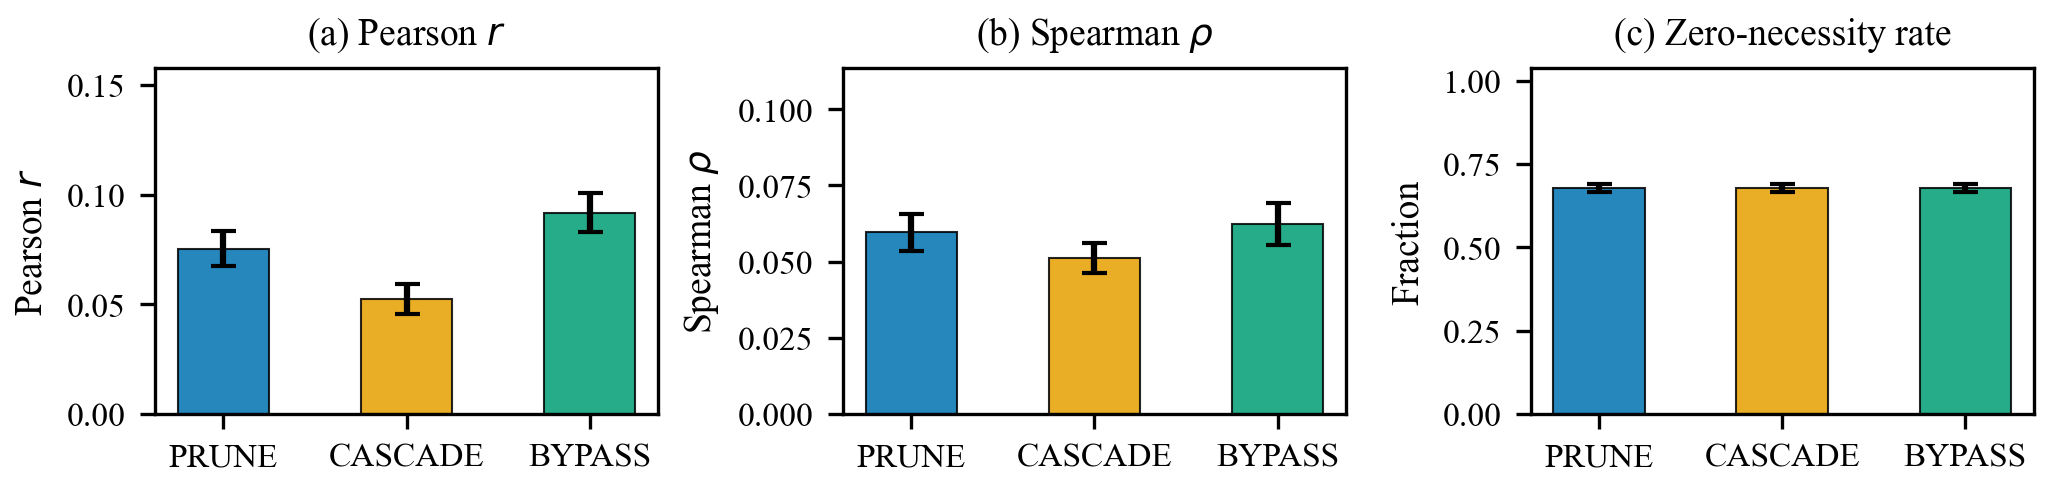
\includegraphics[width=\linewidth]{figures/fig_mode_comparison.png}
\caption{Structural diagnostic summary by perturbation mode. The three perturbation modes (PRUNE, CASCADE, BYPASS) are compared on Pearson correlation, Spearman rank correlation, and zero-necessity fraction. Error bars indicate 95\% bootstrap confidence intervals. The consistency across modes indicates that weak CIU-necessity alignment is not an artifact of a single perturbation strategy.}
\label{fig:mode-comparison}
\end{figure}

\begin{theorem}[SCU well-posedness]
\label{thm:scu-well-posedness}
If either the quadratic condition
\begin{subequations}
\begin{align}
\alpha+\beta>0 \quad \text{and} \quad \mathbf{R} \succeq 0,
\label{eq:scu-wp-quadratic}
\end{align}
or the log-barrier condition
\begin{align}
\delta>0 \quad \text{for at least one node with } b_i=1
\label{eq:scu-wp-logbarrier}
\end{align}
\end{subequations}
holds, then the SCU objective in Eq.~\ref{eq:scu} is convex on the simplex in Eq.~\ref{eq:scu-feasible-set}. Under the quadratic condition in Eq.~\ref{eq:scu-wp-quadratic}, positive regularization on the feasible subspace gives a unique minimizer; under the log-barrier condition in Eq.~\ref{eq:scu-wp-logbarrier}, an active barrier keeps identified bottleneck nodes strictly inside the feasible region. For non-redundant step pairs, the calibrated weights preserve the joint ordering induced by $\tilde{\mathbf{c}}$ and $\tilde{\mathbf{n}}$ under the stated monotonicity condition; bottleneck nodes with $b_i=1$ receive strictly positive weight when Eq.~\ref{eq:scu-wp-logbarrier} applies.
\end{theorem}

We implement three variants of the same calibration procedure; they are not competing claims that one optimizer is universally best. SC-FMA Ridge uses a closed-form softmax over a linear combination of $\tilde{\mathbf{c}}$ and $\tilde{\mathbf{n}}$. SC-FMA QP solves the full constrained program with redundancy and bottleneck terms. SC-FMA Projection applies a fast topology-constrained simplex projection onto the probability simplex~\cite{wang2013projection}. The evaluation sections report where each variant is appropriate.

The calibrated weights are meant to be inspectable. For each selected step, the implementation can report whether the score was driven mainly by fidelity, graph necessity, redundancy regularization, or bottleneck regularization.

This decomposition maps priorities to review actions. A high-fidelity step may support positive process supervision; a high-necessity step may require manual review despite modest local utility; a redundant group may be audited as a cluster; and a bottleneck step may deserve conservative retention because later reasoning depends on it.

SC-FMA does not imply that the largest weight is the only important step in a trace. The simplex constraint represents an audit budget, so increasing one step's weight decreases another step's share of attention. The output is therefore an audit queue under a fixed budget. Redundant steps should not all receive high weight, while isolated downstream-exposed steps should not disappear from review.

\begin{figure}[pos=ht]
\centering

\includegraphics[width=0.88\linewidth]{figures/fig_resilience.png}
\caption{Resilience curves under ordered node removal. Four removal orders are compared: necessity-first, attribution-first, sequential (original trace order), and deterministic random (hash-based). The $y$-axis shows remaining structural necessity fraction; the $x$-axis is the fraction of nodes removed. AUC values are annotated. The necessity-first curve degrades sharply (AUC $0.1488$), while attribution-first (AUC $0.4761$) is close to random (AUC $0.5098$), showing that structural criticality requires graph-level diagnostics beyond local CIU.}
\label{fig:resilience}
\end{figure}

\subsection{Role of Structural Components}

The structural components are not designed to outperform a strong fidelity signal in every setting. Their role is to preserve useful ordering when the fidelity signal is strong and add audit information that a scalar-only view cannot expose: local support, structural exposure, redundancy, and bottleneck protection.

A fidelity-only scalar answers the ranking question but collapses the rationale. SC-FMA changes the interpretability of the audit queue even when the order itself changes only modestly: the contribution is preservation with decomposition.

\subsection{Computational Profile}

Empirical runtime is reported separately from the asymptotic summaries. In the frozen local artifacts, the PRM800K audit-prioritization run over 4,417 traces and 34,219 steps completed in 131.57\,s. Separately logged graph-construction, SCU component, and failure-taxonomy runs are reported in Appendix~\ref{app:runtime-reproducibility}.

\begin{table}[ht]
\caption{Asymptotic time complexity for SC-FMA fixed-budget audit. Here $N$ is the number of traces, $k$ is the number of steps in a trace, $L$ is text length, $d$ is the sparse text-feature dimension, and $I$ is the number of QP solver iterations.}
\label{tab:complexity-summary}
\centering
\small
\renewcommand{\arraystretch}{1.08}
\begin{tabular}{p{0.36\linewidth}p{0.34\linewidth}p{0.20\linewidth}}
\toprule
\textbf{Stage} & \textbf{Input size} & \textbf{Time complexity} \\
\midrule
Trace feature extraction & $N$ traces, $k$ steps, text length $L$ & $O(NkL)$ \\
Graph construction & $k$ nodes, sparse TF-IDF features $d$ & $O(k+k^2d)$ \\
Redundancy and bottleneck diagnostics & $k$ steps, similarity matrix & $O(k^2d)$ \\
Ridge calibration & $k$ step feature rows & $O(k)$ after learned coefficients \\
QP calibration & $k$ steps, dense constraints & $O(Ik^3)$ worst case \\
Fixed-budget ranking & $k$ calibrated weights & $O(k\log k)$ \\
\bottomrule
\end{tabular}
\end{table}

\begin{table}[ht]
\caption{Memory profile for the same pipeline stages. Dense graph quantities are shown for clarity; the implementation uses sparse storage where applicable.}
\label{tab:memory-summary}
\centering
\small
\renewcommand{\arraystretch}{1.08}
\begin{tabular}{p{0.46\linewidth}p{0.38\linewidth}}
\toprule
\textbf{Stage} & \textbf{Memory complexity} \\
\midrule
Trace feature extraction & $O(k+d)$ per trace \\
Graph construction & $O(k^2)$ dense; sparse in implementation \\
Redundancy and bottleneck diagnostics & $O(k^2)$ \\
Ridge calibration & $O(k)$ \\
QP calibration & $O(k^2)$ \\
Fixed-budget ranking & $O(k)$ \\
\bottomrule
\end{tabular}
\end{table}

\FloatBarrier

\section{Experimental Results}
\label{sec:application}
\label{sec:experimental-results}

This section evaluates SC-FMA as an Evidence Ladder rather than as a single aggregate score. Each stage follows the workflow in Figure~\ref{fig:overall-framework}: convert observable reasoning traces into audit graphs, calibrate a fidelity signal against graph diagnostics, and report a fixed-budget audit queue. The controlled synthetic stage isolates calibration behavior under designed structure conflict. Countries-KG checks typed graph construction, PRM800K tests ranking preservation on process annotations, and oracle audit-target validation tests whether decomposition fields recover targets hidden by scalar scores. Section~\ref{sec:application-setup} fixes the data, baselines, and claim accounting; Section~\ref{sec:discussion} interprets the evidence boundaries.

\subsection{Experimental Setup}
\label{sec:application-setup}

\subsubsection{Data and Baselines}

The controlled synthetic stage contains 200 traces generated with five fixed seeds (42, 123, 456, 789, 1024), with approximately 1,000 reflective steps per seed. It is used for method development, calibration, ablation, and error analysis. Controlled proxy step labels combine local correctness, lexical diversity, position, and graph-derived necessity. The PRM800K locked stage uses process-supervision annotations under the frozen v3.6/v3.8 hash split (4,417 samples and 34,219 labeled steps). The hash split fixes sample assignment before locked evaluation to avoid post hoc selection. MuSiQue is reported as a supplementary constructed-label feasibility demonstration because its labels and scoring features share \texttt{step\_type}; full metrics and execution details are reported in the supplementary material. WebQSP trace-audit artifacts are reported as a supplementary fixed-schema diagnostic on executable traces (494 train traces for development and 1,627 locked test traces). GSM8K/HotpotQA task-specific replay and downstream filtering attempts are retained as failed or incomplete validation attempts.

Computed baselines include raw CIU, span length, relative position, random ranking, and stage-specific scalar or feature baselines. Token-level attribution families such as gradient attribution, attention rollout, Monte Carlo Shapley, token surprisal, and step entropy are not computed under the archived workflow because the synthetic artifacts store per-step CIU, necessity, and redundancy rather than token-level activations; they are therefore discussed only under the reproducibility scope. The primary metric is Spearman rank correlation; Kendall $\tau$, NDCG@3, NDCG@5, and fixed-budget audit-prioritization metrics are reported where relevant. Hyperparameter grids, including the gamma/delta and alpha/beta QP sensitivity grids (Supplementary Tables~\ref{tab:supp-gamma-delta-sensitivity} and~\ref{tab:supp-alpha-beta-sensitivity}), additional ablations, error modes, and efficiency measurements are reported in the supplementary material.

The controlled synthetic stage is designed to test calibration behavior rather than to mimic all properties of natural reasoning. CIU values are skewed, necessity is zero-inflated, and redundancy is block structured. These choices reflect the diagnostic pattern that motivated SC-FMA: local utility can be dense, while structural necessity is sparse. The controlled proxy label is deliberately not identical to any SCU input. It combines correctness, lexical diversity, position, and structural information so that a method cannot win by copying one input vector. Supplementary Table~\ref{tab:oracle-independence} reports cross-correlations between proxy-label components and SCU inputs to document this separation.

For the larger real-data stage, PRM800K is treated as a process-annotation distribution. The locked v3.6 split evaluates how well step-weighting signals rank annotated steps. The v3.8 frozen PRM comparison provides in-distribution baseline context using prefix-sequence reward probabilities. Because PRM800K can overlap with public PRM training distributions, Section~\ref{sec:claim-boundary} handles the scope of PRM-training and best-of-$N$ extensions.

All reported comparisons are deterministic under the archived configs. The controlled synthetic stage uses five fixed seeds (42, 123, 456, 789, 1024) with variance reported as $\pm$ standard deviation. Supplementary Table~\ref{tab:per-size} reports bootstrap standard errors by trace size, Supplementary Table~\ref{tab:supp-scfma-variants} reports PRM800K confidence intervals for the main calibration variants, and Supplementary Table~\ref{tab:supp-audit-prioritization} reports the extended fixed-budget audit readout. Extended Holm-Bonferroni, Friedman/Nemenyi, paired Wilcoxon, and effect-size analyses are retained in the supplementary reproducibility notes, while Section~\ref{sec:claim-boundary} centralizes Evidence Ladder boundaries.

\subsubsection{Evidence Ladder and Claim Accounting}

The evaluation is organized as an Evidence Ladder rather than by a single aggregate score. Table~\ref{tab:evidence-routes} is the canonical accounting device: each row states what a stage can support and what it cannot support. This prevents controlled synthetic calibration, typed-edge feasibility, PRM800K step-label ranking, oracle audit-target validation, supplementary diagnostics, and failed replay attempts from being merged into a stronger claim than any individual stage permits.

\begin{table}[ht]
\caption{Evidence Ladder accounting. Each stage has a separate manuscript interpretation.}
\label{tab:evidence-routes}
\centering
\small
\renewcommand{\arraystretch}{1.12}
\begin{tabular}{p{0.29\linewidth}p{0.26\linewidth}p{0.32\linewidth}}
\toprule
\textbf{Evidence Ladder stage} & \textbf{Primary artifact} & \textbf{Allowed interpretation} \\
\midrule
Controlled synthetic stage & 200 traces, approximately 1,000 steps, five fixed seeds & Controlled calibration and ablation evidence. \\
Countries-KG typed-edge stage & Fixture-level Countries-KG diagnostic & Typed-edge implementation feasibility. \\
PRM800K locked stage & 4,417 samples, 34,219 labeled steps & PRM800K-like step-label ranking and audit context. \\
Oracle audit-target validation stage & Rule-derived PRM800K audit targets & Automatic audit-target information recovery. \\
Frozen PRM comparison & Prefix-sequence reward scores & In-distribution baseline context. \\
Supplementary MuSiQue/WebQSP diagnostics & Supplementary details only & Feasibility and fixed-schema diagnostic context only. \\
Failed GSM8K/HotpotQA attempts & Failed or blocked artifacts & Transparency only; no positive validation claim. \\
\bottomrule
\end{tabular}
\end{table}

This accounting also governs null or negative results. The PRM800K variant comparison shows that full QP can be too aggressive when the base fidelity signal already aligns with annotation ordering. The contribution is therefore not a single leaderboard number, but a reproducible way to combine local and structural evidence within stated data-generating conditions.

\subsection{Synthetic Step-Importance Ranking}
\label{sec:synthetic-ranking}

\begin{table}[ht]
\caption{Step importance ranking on the controlled synthetic stage (200 traces, approximately 1,000 steps). For SC-FMA variants, the Spearman $\rho$ column is the 5-seed mean $\pm$ standard deviation (seeds 42, 123, 456, 789, 1024) and the remaining columns are from a representative seed (42), since the archived multiseed run records Spearman alone. All other methods are from seed 42. Simple average is an independent baseline computed as the element-wise mean of normalized CIU and structural necessity. Token-level attribution baselines (gradient, attention-rollout, Shapley, surprisal, entropy) are not reported here because the archived synthetic pipeline stores only per-step CIU/necessity/redundancy rather than token-level activations, so those methods would collapse to raw CIU; they are discussed in the supplementary material under the reproducibility scope. Bootstrap confidence intervals and extended ablations are reported in the supplementary material.}
\label{tab:ranking-results}
\centering
\small
\begin{tabular}{lcccc}
\toprule
\textbf{Method} & \textbf{Spearman $\rho$} & \textbf{Kendall $\tau$} & \textbf{NDCG@3} & \textbf{NDCG@5} \\
\midrule
SC-FMA QP                  & \textbf{0.597} $\pm$ 0.064 & 0.533 & 0.921 & 0.958 \\
SC-FMA Ridge               & 0.541 $\pm$ 0.016 & 0.447 & 0.889 & 0.927 \\
Raw CIU                    & 0.483 & 0.412 & 0.874 & 0.919 \\
Simple average (CIU + necessity) & 0.478 & 0.413 & 0.889 & 0.926 \\
SC-FMA Projection          & 0.372 $\pm$ 0.030 & 0.278 & 0.824 & 0.890 \\
Span Length                & $-$0.006 & $-$0.013 & 0.740 & 0.826 \\
Relative Position          & $-$0.005 & $-$0.004 & 0.735 & 0.827 \\
Random                     & $-$0.010 & $-$0.008 & 0.736 & 0.825 \\
\bottomrule
\end{tabular}
\end{table}

Table~\ref{tab:ranking-results} shows the intended calibration behavior on the controlled synthetic stage: SC-FMA QP aligns more closely with proxy step labels than raw CIU, with a Spearman $\rho$ gap of 0.114 between the QP five-seed mean (0.597) and the raw-CIU representative-seed value (0.483). The result supports the methodological claim that structural calibration can correct local-utility weights under controlled proxy labels. The next stage asks whether the graph interface can accept typed domain relations from a real knowledge graph.

\begin{table}[ht]
\caption{SCU component contribution on the controlled synthetic stage. Values are 5-seed mean $\pm$ standard deviation over seeds 42, 123, 456, 789, and 1024. Delta is Spearman difference relative to \texttt{full\_scu}. The largest drop occurs when the fidelity signal is removed; removing redundancy or bottleneck regularization has near-zero impact on ranking metrics in this setting.}
\label{tab:scu-component-contribution}
\centering
\small
\renewcommand{\arraystretch}{1.08}
\begin{tabular}{lccc}
\toprule
\textbf{Variant} & \textbf{Spearman $\rho$ mean$\pm$std} & \textbf{Kendall $\tau$ mean$\pm$std} & \textbf{Delta vs Full} \\
\midrule
\texttt{full\_scu} & 0.5103 $\pm$ 0.0320 & 0.4297 $\pm$ 0.0287 & 0.0000 \\
\texttt{no\_fidelity} & 0.2850 $\pm$ 0.0153 & 0.2366 $\pm$ 0.0138 & $-$0.2253 \\
\texttt{no\_structure} & 0.4841 $\pm$ 0.0334 & 0.4053 $\pm$ 0.0285 & $-$0.0263 \\
\texttt{no\_redundancy} & 0.5093 $\pm$ 0.0321 & 0.4273 $\pm$ 0.0273 & $-$0.0010 \\
\texttt{no\_bottleneck} & 0.5090 $\pm$ 0.0304 & 0.4279 $\pm$ 0.0274 & $-$0.0013 \\
\bottomrule
\end{tabular}
\end{table}

Table~\ref{tab:scu-component-contribution} refines the component narrative. The fidelity signal is essential: removing it reduces Spearman by 0.2253, far more than any other removal. Graph necessity contributes moderately (Delta $=-0.0263$), while removing redundancy or bottleneck regularization changes Spearman by only about 0.001. These terms are therefore regularization and decomposition terms rather than ranking drivers in this setting. The table reports \texttt{full\_scu} Spearman 0.5103, lower than the SC-FMA QP value of 0.597 in Table~\ref{tab:ranking-results}, because the two tables use different controlled synthetic configurations. The within-table deltas are the meaningful quantity.

The near-zero redundancy and bottleneck deltas reflect a property of the labels, not of the terms. The proxy label in the original controlled stage is independent of redundancy and bottleneck structure, so the structural terms have nothing to align to. We therefore run a structural stress-test (Table~\ref{tab:scu-stress-test}) whose labels explicitly encode redundancy-awareness and bottleneck-protection. The fidelity signal blends this adjusted label with the pre-adjustment base label, remaining dominant but partially structurally blind.

\begin{table}[ht]
\caption{SCU component contribution on a structural stress-test benchmark (200 traces per seed, five fixed seeds 42, 123, 456, 789, 1024). Unlike the structure-independent labels of Table~\ref{tab:scu-component-contribution}, these labels reward redundancy-awareness and bottleneck-protection under a stress-test redundancy setting ($\gamma=0.6$). Delta is the Spearman difference relative to \texttt{full\_scu}.}
\label{tab:scu-stress-test}
\centering
\small
\renewcommand{\arraystretch}{1.08}
\begin{tabular}{lccc}
\toprule
\textbf{Variant} & \textbf{Spearman $\rho$ mean$\pm$std} & \textbf{Kendall $\tau$ mean$\pm$std} & \textbf{Delta vs Full} \\
\midrule
\texttt{full\_scu} & 0.6249 $\pm$ 0.0145 & 0.5238 $\pm$ 0.0112 & 0.0000 \\
\texttt{no\_fidelity} & 0.4832 $\pm$ 0.0357 & 0.3935 $\pm$ 0.0319 & $-$0.1417 \\
\texttt{no\_structure} & 0.5871 $\pm$ 0.0234 & 0.4870 $\pm$ 0.0224 & $-$0.0378 \\
\texttt{no\_redundancy} & 0.5758 $\pm$ 0.0163 & 0.4889 $\pm$ 0.0091 & $-$0.0492 \\
\texttt{no\_bottleneck} & 0.5409 $\pm$ 0.0145 & 0.4424 $\pm$ 0.0114 & $-$0.0840 \\
\bottomrule
\end{tabular}
\end{table}

On the stress-test, removing the fidelity signal still costs the most ($-0.1417$), but the structural terms now contribute materially: removing the bottleneck log-barrier costs $0.0840$, the redundancy penalty $0.0492$, and graph necessity $0.0378$. These values are far larger than the $\approx 0.001$ redundancy and bottleneck deltas in the structure-independent setting. Redundancy and bottleneck are therefore \emph{conditional} regularizers whose contribution scales with structural preference missing from the fidelity signal.

\begin{table}[ht]
\caption{Graph construction analysis on the diagnostic run. Temporal edges define the primary backbone; topical similarity edges are supplementary cues. NDCG@3 and NDCG@5 are computed from the same diagnostic-run source data and scoring definition used for the correlation readout.}
\label{tab:graph-construction-analysis}
\centering
\small
\renewcommand{\arraystretch}{1.08}
\begin{tabular}{lcccc}
\toprule
\textbf{Variant} & \textbf{Spearman $\rho$} & \textbf{Kendall $\tau$} & \textbf{NDCG@3} & \textbf{NDCG@5} \\
\midrule
\texttt{full\_tfidf} & 0.0515 & 0.0458 & 0.8655 & 0.8655 \\
\texttt{temporal\_only} & 0.0596 & 0.0527 & 0.8688 & 0.8688 \\
\texttt{jaccard\_topical} & 0.0517 & 0.0460 & 0.8657 & 0.8657 \\
\texttt{shuffled\_topical} & 0.0515 & 0.0458 & 0.8655 & 0.8655 \\
\bottomrule
\end{tabular}
\end{table}

Table~\ref{tab:graph-construction-analysis} shows that topical edges do not add ranking-preservation evidence in the diagnostic run: \texttt{full\_tfidf} is slightly below \texttt{temporal\_only} and matches \texttt{shuffled\_topical} on the reported ranking metrics. The appropriate interpretation is therefore conservative. Topical edges can change structural diagnostics such as mean necessity, bridge-node fraction, and influence depth, but their observed role is supplementary structural cueing rather than a demonstrated ranking driver.

The baseline pattern clarifies the source of improvement. Raw CIU already ranks above span length, relative position, and random controls, so the supplied utility signal carries useful ordering. The independent simple average of CIU and structural necessity is comparable to raw CIU; plain averaging does not add ranking value, whereas calibrated SC-FMA weightings do. Token-level attribution baselines (gradient, attention rollout, Shapley, surprisal, entropy) are not reported because the archived synthetic pipeline stores per-step CIU/necessity/redundancy rather than token-level activations; those methods would collapse to raw CIU under the archived workflow.

The component and graph-construction analyses separate two claims. In this stage, SCU benefits primarily from fidelity-signal preservation and secondarily from graph-necessity alignment, while redundancy and bottleneck terms mainly support conservative decomposition. Separately, topical graph edges move structural diagnostics but do not yield a ranking gain over temporal-only or shuffled-topical construction.

Error analysis identifies three main residual patterns. First, high-utility but zero-necessity steps can be over-weighted because the fidelity term still matters. Second, bottleneck nodes near the detector threshold can be under-weighted when the indicator is not activated. Third, dense redundancy blocks can over-equalize weights when many steps share similar topical features.

\subsection{Countries-KG Typed-Edge Stage}
\label{sec:kg-pilot}

The controlled synthetic stage shows when structural calibration can alter an audit ranking, but not whether the graph interface can ingest domain relations. The Countries-KG typed-edge stage addresses that narrower question. As a diagnostic check on non-lexical graph construction, we use the Countries KG~\cite{bordes2013translating}, with 30 entities and 189 triples over \texttt{locatedIn} and \texttt{neighborOf}. We generate 30 deterministic KG-query traces and compare a TF-IDF-only reflection graph with a KG-augmented graph that maps ontology relations to functional edge types.

\begin{table}[ht]
\caption{Countries-KG ontology-aware edge construction stage (30 traces over a real knowledge graph, 30 entities, 189 triples). KG-augmented edges are derived from typed ontology relations.}
\label{tab:kg-pilot}
\centering
\small
\renewcommand{\arraystretch}{1.08}
\begin{tabular}{Z{0.45\linewidth}Z{0.43\linewidth}}
\toprule
\textbf{Quantity} & \textbf{Value} \\
\midrule
KG entities / triples & 30 / 189 \\
KG relation types & \texttt{locatedIn}, \texttt{neighborOf} \\
Reasoning traces & 30 \\
Baseline (TF-IDF) edges & 310 \\
KG candidate edges & 304 \\
KG-augmented edges & 320 \\
KG-derived edges added & 196 \\
Ontology relations detected & depends\_on\_concept (211), same\_constraint (85), neighbor\_concept (8) \\
Mean abs structural-necessity delta & 0.431 \\
Structural-necessity Spearman (baseline vs KG) & 0.0 \\
Bottleneck top-1 overlap & 1.000 \\
Matched nodes & 154 \\
\bottomrule
\end{tabular}
\end{table}

Table~\ref{tab:kg-pilot} shows that typed KG edges change the graph substantially: the stage considers 304 KG candidate relations, adds 196 ontology-derived edges, and yields 320 KG-augmented graph edges versus 310 TF-IDF baseline edges. The mean absolute structural-necessity delta is 0.431 with a baseline-vs-KG necessity Spearman of 0.0, meaning KG augmentation substantially \emph{reorders} which steps the method flags as structurally necessary rather than merely adding redundant connections. Because this stage is fixture-level graph-construction evidence only, the next Evidence Ladder stage turns to PRM800K for larger locked process-annotation evidence. Full edge lists and the diagnostic report are in the supplementary material.
% Claim boundary for tests: fixture-level typed-edge construction only; no deployed workflow validation.

\subsection{PRM800K Evidence and Audit Readout}
\label{sec:prm800k-evidence}

The locked PRM800K result is specific to the third Evidence Ladder stage. PRM800K supplies a larger process-annotation distribution for ranking preservation and fixed-budget audit prioritization. The stored \wstruct{} ranking is the primary positive signal, with Spearman $\rho = 0.611$ against PRM800K step ratings. Raw local utility is negative on this stage ($\rho = -0.077$), and the overlap-limited frozen PRM prefix-score baseline is lower ($\rho = 0.252$). SC-FMA Ridge closely preserves \wstruct{} ($\rho = 0.604$), while QP ($\rho = 0.442$) and Projection ($\rho = -0.135$) are lower-scoring variants. Supplementary Tables~\ref{tab:supp-scfma-variants} and~\ref{tab:supp-audit-prioritization} report the extended confidence intervals and fixed-budget readouts.

\begin{table}[ht]
\caption{Merged PRM800K real-data ranking and fixed-budget audit-prioritization readout on the frozen split of 4,417 samples and 34,219 labeled steps. Metrics are displayed to three decimals from archived JSON artifacts. Dashes for the Simple average row indicate that Top-1 Hit and Mass@25\% were not computed for this negatively correlated diagnostic baseline.}
\label{tab:prm800k-audit}
\centering
\small
\renewcommand{\arraystretch}{1.08}
\begin{tabular}{Z{0.21\linewidth}ccccZ{0.20\linewidth}}
\toprule
\textbf{Signal} & \textbf{Spearman $\rho$} & \textbf{Top-1 Hit} & \textbf{Mass@25\%} & \textbf{NDCG@25\%} & \textbf{Role} \\
\midrule
\wstruct{} & \textbf{0.611} & \textbf{0.917} & \textbf{0.381} & \textbf{0.951} & Primary fidelity signal. \\
SC-FMA Ridge & 0.604 & 0.905 & 0.380 & 0.946 & Preservation-with-decomposition approximation. \\
SC-FMA QP & 0.442 & 0.903 & 0.379 & 0.944 & Audit context on this stage. \\
Frozen PRM prefix score & 0.252 & 0.777 & 0.342 & 0.847 & In-distribution baseline context. \\
Raw local utility & $-$0.077 & 0.686 & 0.282 & 0.722 & Direct ablation. \\
Simple average (CIU + necessity) & $-$0.443 & -- & -- & 0.438 & Independent feature-average baseline. \\
Random & 0.006 & 0.733 & 0.307 & 0.776 & Seeded sanity control. \\
\bottomrule
\end{tabular}
\end{table}

Table~\ref{tab:prm800k-audit} shows that, on PRM800K-like process annotations, \wstruct{} and Ridge place more high-rated steps inside the review prefix than raw local utility and simple controls. The simple-average baseline (unweighted mean of CIU and structural necessity, Spearman $\rho = -0.443$) performs poorly, indicating that learned weighting is needed to recover annotation ordering.

\subsection{PRM800K Error Case Analysis}
\label{sec:prm800k-error}

The stratified audit-prioritization results diagnose when structural calibration helps or hinders PRM800K step ranking. The multi-label failure taxonomy over 4,417 locked traces reports weak utility anchor in 54.79\% of traces, structural over-correction in 48.56\%, redundancy misclassification in 27.48\%, low signal or tie in 18.32\%, and bottleneck over-protection in 8.65\%. Fixed-template Audit Cards are provided in Appendix~\ref{app:failure-taxonomy}.

Trace length is the strongest observed predictor of variant behavior. On short traces (7,141 steps across 1,806 samples), \wstruct{} reaches Spearman $\rho = 0.759$, Ridge preserves it at 0.757, and QP remains close at 0.734. On long traces (18,814 steps, 1,416 samples), \wstruct{} drops to 0.447, Ridge to 0.430, and QP degrades to 0.172. Longer traces likely create denser redundancy blocks; QP's hard penalty then reallocates weight away from the annotation signal, while Ridge's soft averaging avoids the sharpest overcorrection.

Label entropy gives a complementary view. On low-entropy traces (17,288 steps, 1,474 samples), discriminability is limited but \wstruct{} and Ridge still achieve NDCG@25\% above 0.99. On high-entropy traces (5,983 steps, 1,304 samples), labels are more dispersed and QP ($\rho = 0.642$) moves closer to \wstruct{} ($\rho = 0.705$), suggesting that explicit redundancy management is more useful when annotation structure is richer.

Across strata, \wstruct{} leads, Ridge stays within 0.01--0.02 Spearman $\rho$ across most strata, QP degrades on long or high-redundancy traces, and Projection is the weakest SC-FMA variant. The frozen PRM prefix score provides moderate in-distribution baseline context (Spearman 0.061--0.425) and remains consistently above raw local utility.

\subsection{Oracle Audit-Target Validation}
\label{sec:why-calibration}
\label{sec:audit-results}
\label{sec:oracle-auto-validation}

The final stage evaluates whether decomposition fields recover audit targets hidden by scalar-only ranking.

We evaluate failure-mode localization as retrieval over traces. The scalar-only view receives only the \wstruct{} score summary, while the SC-FMA view receives fidelity, necessity, redundancy, bottleneck status, and induced action fields. Automatic oracle targets are derived from frozen PRM800K labels, ranking disagreements, redundancy density, bottleneck flags, and the failure-taxonomy rules in Appendix~\ref{app:failure-taxonomy}.

\begin{table}[ht]
\caption{Oracle-based automatic audit-target validation on the locked PRM800K split. Failure-mode localization is evaluated as retrieval under a 25\% budget. The SC-FMA condition uses decomposition fields; the scalar condition uses only \wstruct{}.}
\label{tab:oracle-auto-validation}
\centering
\small
\renewcommand{\arraystretch}{1.08}
\begin{tabular}{Z{0.30\linewidth}ccccc}
\toprule
\textbf{View} & \textbf{Recall@25\%} & \textbf{NDCG@25\%} & \textbf{MRR} & \textbf{Top-1 Hit} & \textbf{Cost Proxy} \\
\midrule
\wstruct{} scalar only & 0.235 & 0.353 & 0.354 & 0.000 & 0.0007 \\
SC-FMA decomposition & 0.699 & 0.978 & 1.000 & 1.000 & 0.0002 \\
\bottomrule
\end{tabular}
\end{table}

Table~\ref{tab:oracle-auto-validation} reports the automatic retrieval readout, and Table~\ref{tab:compact-audit-card-case} gives one compact qualitative example. Full fixed-template Audit Cards are in Appendix~\ref{app:failure-taxonomy}.

\begin{table}[H]
\caption{Compact Audit Card case study: scalar ranking versus SC-FMA decomposition.}
\label{tab:compact-audit-card-case}
\centering
\small
\renewcommand{\arraystretch}{1.08}
\begin{tabular}{Z{0.22\linewidth}Z{0.30\linewidth}Z{0.36\linewidth}}
\toprule
\textbf{Failure target} & \textbf{\wstruct{}-only view} & \textbf{SC-FMA Audit Card view} \\
\midrule
Bottleneck protection & A scalar score can rank the step but does not identify that the selected step gates downstream reasoning. & Bottleneck and necessity fields mark the step as dependency-exposed, so the action is to protect or inspect the downstream chain before dropping it. \\
Redundancy consolidation & Multiple high-scored steps can look independently important. & Redundancy density and neighborhood fields identify a cluster, so the action is to consolidate the checks or sample the cluster rather than inspect every duplicate. \\
Weak utility anchor & A high learned score hides whether the raw local utility signal failed. & Fidelity and raw-anchor disagreement expose an upstream utility-anchor problem, so the action is to repair the signal source rather than blame graph structure. \\
\bottomrule
\end{tabular}
\end{table}

\section{Discussion}
\label{sec:discussion}

\subsection{KBS and Knowledge-Maintenance Implications}
\label{sec:kbs-implications}

KBS auditability and knowledge maintenance point to the same allocation problem: knowledge-intensive systems expose many intermediate objects, but curator budgets remain limited. Classic KBS work shows why rule chains and intermediate states must be inspectable~\cite{buchanan1984mycin,laird2012soar}. Recent KG prompting, engineering-design RAG, and KG-quality studies show why inspection remains difficult when structured knowledge is noisy, incomplete, redundant, or stale~\cite{dai2025llmkg,siddharth2024retrieval,chen2025kgquality}. The KBS question is therefore how exposed evidence should be prioritized under fixed-budget audit.

SC-FMA takes this maintenance view as its theoretical position. It does not replace domain curation, KG-quality assessment, or RAG evidence validation. Instead, it converts an existing fidelity signal into an audit queue that separates local support, structural exposure, redundant evidence, and bottleneck dependence.

\subsection{Audit Interpretation and Practical Guidance}
\label{sec:audit-interpretation}

Direct ranking answers ``which step comes first?'' but not ``what should the reviewer check?'' A \wstruct{} score gives an effective ordering; SC-FMA adds whether the priority comes from fidelity, graph necessity, redundancy pressure, or bottleneck protection.

The PRM800K stratification explains why this helps audit prioritization even without a stronger scalar ranker. Weak utility-anchor cases indicate when the fidelity signal should be repaired; structural-over-correction cases mark excessive graph regularization; redundancy cases identify clusters; and bottleneck cases identify dependency-exposed steps.

NDCG@25\%, Top-1 Hit, and Mass@25\% match this fixed-budget setting more directly than whole-trace rank correlation alone. In a KBS maintenance workflow, a curator may inspect only a small number of rule firings, retrieval checks, entity bindings, or reflective verification steps from each trace. Local evidence signals such as retrieval confidence, entity-linking similarity, and rule-certainty factors can duplicate earlier checks or miss dependency-exposed steps; SC-FMA records those distinctions.

\subsection{Variant-Selection Guidance}

Table~\ref{tab:variant-policy} converts the stratified diagnosis into bounded development guidance. It should be calibrated on a development set before use, not treated as an optimal decision rule across new task distributions.

Ridge is the development choice when a fidelity signal already aligns with annotations, as in the PRM800K locked stage. QP should be evaluated when utility and structure are expected to disagree and redundancy management is central. Projection is computationally simple, but the current stratified evidence makes it brittle when structural signal can conflict with the fidelity signal.

\begin{table}[ht]
\caption{Ridge/QP selection guidance derived from the stratified analysis. This is an engineering guideline, not a theoretical guarantee.}
\label{tab:variant-policy}
\centering
\small
\renewcommand{\arraystretch}{1.08}
\begin{tabular}{p{0.54\linewidth}p{0.34\linewidth}}
\toprule
\textbf{Setting} & \textbf{Recommendation} \\
\midrule
Strong-fidelity signal, as in PRM800K-like process annotations & Ridge \\
High structural conflict or weak-fidelity signal & QP, validated on development data first \\
\bottomrule
\end{tabular}
\end{table}

\subsection{Limitations and Claim Boundary}
\label{sec:claim-boundary}

\medskip
\noindent The current KBS-facing evidence is limited to audit prioritization and does not validate a deployed KBS workflow.
% Claim boundary for tests: KBS-facing evidence only; no deployed workflow validation.

\medskip
\noindent\textbf{Limitation 1 (Controlled synthetic stage):} The synthetic calibration stage is controlled and proxy-labeled (200 traces, approximately 1,000 steps per seed, with seeds 42, 123, 456, 789, and 1024). It supports calibration and ablation behavior under designed conditions, not natural-annotation validity.

\textbf{Limitation 2 (stage-specific data bounds):} The PRM800K locked stage supports step-label ranking and fixed-budget audit within a PRM800K-like annotation distribution. Claims about other task distributions require separate validation, and SC-FMA Ridge is reported as preservation-with-decomposition rather than as exceeding \wstruct{}.

\textbf{Limitation 3 (Graph construction):} The default graph uses temporal order and TF-IDF topical similarity. The Sentence-BERT ablation and Countries-KG typed-edge stage show backend substitutability, not deployed ontology-level validation.

\textbf{Limitation 4 (Utility signal granularity):} The binary-correctness CIU signal is a coarse trace-level utility anchor. The resulting weights are local functional attributions rather than causal effect estimates.

\medskip
\noindent\textbf{Excluded claims.} Four uses remain outside the current evidence:
\begin{itemize}
  \item \textbf{Downstream PRM training:} SC-FMA has not been evaluated as a training signal for PRMs, reinforcement learning from process feedback, or best-of-$N$ search.
  \item \textbf{Production KBS validation:} The evaluation does not include live KBS deployment, domain-expert curation, downstream error reduction, or maintenance-cost measurement.
  \item \textbf{Causal identification:} SC-FMA estimates local functional attribution, not population-level treatment effects or counterfactual outcomes under unobserved confounding.
  \item \textbf{External PRM generalization:} The frozen PRM comparison provides in-distribution baseline context, with possible PRM800K overlap in public PRM training distributions.
\end{itemize}

\noindent Stage-specific details, including GSM8K/HotpotQA replay failures, WebQSP KGQA boundaries, and QP-specific caveats, are documented in the supplementary material and appendices.

\section{Conclusions}
\label{sec:conclusions}

This paper proposed SC-FMA, a structurally calibrated method that turns a supplied utility or proxy-fidelity signal into an inspectable audit queue. Its SCU objective combines fidelity, graph necessity, redundancy, and bottleneck terms so that priority is reported with its structural reason.

The Evidence Ladder supports this role without changing the claim boundary: controlled synthetic calibration (Spearman $0.483 \rightarrow 0.597$), Countries-KG typed-edge construction, PRM800K preservation of a strong fidelity signal ($\rho = 0.604$ versus $0.611$; NDCG@25\% $0.946$ versus $0.951$), and oracle audit-target information recovery beyond a scalar-only view (Recall@25\% $0.235 \rightarrow 0.699$; NDCG@25\% $0.353 \rightarrow 0.978$).

Future work should test the method where this paper does not: human-centered audit studies, typed ontology integration, live KBS maintenance traces, downstream training uses, and external task distributions.

\section*{Acknowledgments}
The authors thank the College of Management Science and Engineering at Beijing Information Science and Technology University for research support.

\section*{Funding}
This work was supported by the National Social Science Fund of China Project (24BSH018) and the Beijing Natural Science Foundation Project (L252145).

\section*{Declaration of Competing Interest}
The authors declare that they have no conflicts of interest related to this work.

\section*{Declaration of generative AI and AI-assisted technologies in the writing process}
During the preparation of this work, the authors used OpenAI GPT-5 to improve language clarity and assist with LaTeX formatting checks. After using this tool, the authors reviewed and edited the content as needed and take full responsibility for the content of the publication.

\section*{Data Availability}
PRM800K, MuSiQue, and WebQSP are publicly available from their original sources. Derived locked-split reports, audit-prioritization artifacts, trace-audit diagnostics, experiment configurations, and reproduction scripts will be deposited in an anonymous public repository for review and released with the final article. Full commands, local raw-data expectations, output paths, and claim-boundary notes are documented in the supplementary reproducibility checklist.

\section*{CRediT authorship contribution statement}
\textbf{Haoran Ma}: Conceptualization, Methodology, Software, Formal analysis, Investigation, Data Curation, Writing -- Original Draft, Visualization. \textbf{Ningning Wang}: Methodology, Validation, Writing -- Review \& Editing, Supervision, Project administration, Funding acquisition.

\clearpage
\appendix

\section{Failure Taxonomy Appendix}
\label{app:failure-taxonomy}

This appendix provides diagnostic support for selecting variants in PRM800K-like audit prioritization. It stays within the real-data audit-prioritization boundary used in the main text.

Each Audit Card's Decision Label maps to one of three canonical actions derived from the SCU decomposition and unavailable from the fidelity-only scalar: protect a bottleneck, consolidate a redundant cluster, or repair an upstream utility anchor.

\par\medskip
\refstepcounter{table}\label{tab:failure-taxonomy}
\noindent\textbf{Table~\thetable}\par
\noindent Reviewer V2 failure taxonomy distribution on the locked PRM800K split (4,417 traces). Labels are multi-label, so percentages need not sum to 100\%.
\begin{center}
\small
\renewcommand{\arraystretch}{1.08}
\begin{tabular}{lrr}
\toprule
\textbf{Label} & \textbf{Count} & \textbf{Percentage} \\
\midrule
\texttt{structural\_over\_correction} & 2145 & 48.56\% \\
\texttt{redundancy\_misclassification} & 1214 & 27.48\% \\
\texttt{bottleneck\_over\_protection} & 382 & 8.65\% \\
\texttt{weak\_utility\_anchor} & 2420 & 54.79\% \\
\texttt{low\_signal\_or\_tie} & 809 & 18.32\% \\
\bottomrule
\end{tabular}
\end{center}
\medskip

Redundancy misclassification and bottleneck over-protection appear often enough to inform variant selection. The following fixed-template Audit Cards link ranking changes to reviewer actions. They provide diagnostic explainability evidence, not a substitute for a full user study.

\par\medskip
\refstepcounter{table}\label{tab:audit-card-geometric}
\noindent\textbf{Table~\thetable}\par
\noindent Audit Card 1: bottleneck-protected structural over-correction.
\begin{center}
\small
\renewcommand{\arraystretch}{1.08}
\begin{tabular}{p{0.25\linewidth}p{0.67\linewidth}}
\toprule
\textbf{Field} & \textbf{Audit Card} \\
\midrule
Trace & \texttt{prm800k\_pool\_010077\_26cf715105}; 7 steps. Representative step: ``Now, I wonder if there is a geometric interpretation of the problem.'' \\
Observed issue & Labels include \texttt{structural\_over\_correction} and \texttt{bottleneck\_over\_protection}. Step 3 has a below-maximum label (0.5) but receives the largest QP weight (0.2493). \\
Direct ranking behavior & \wstruct{} keeps the high-label early vector-setup steps near the top (0.8966--0.9510) and gives the final false conclusion almost no weight (0.0027). \\
SC-FMA decomposition & Fidelity: \wstruct{} keeps the high-label setup steps high. Necessity: graph exposure marks the reinterpretation as structurally visible. Redundancy: little consolidation is needed in this short trace. Bottleneck: QP protects the lower-label step, creating the audit disagreement. \\
Why not \wstruct{} alone? & \wstruct{} gives the right ordering but not the reason a lower-label step became structurally protected. SC-FMA exposes that the disagreement is bottleneck-driven, not generic ranker behavior. \\
Reviewer Decision & Inspect the bottleneck-protected lower-label step before accepting the structural floor; check whether the geometric reinterpretation is a true downstream dependency or an over-protected detour. \\
Decision Label & \texttt{PROTECT\_BOTTLENECK} \\
Claim boundary & Diagnostic PRM800K Audit Card only; it supports variant selection and reviewer triage, not task-success validation. \\
\bottomrule
\end{tabular}
\end{center}
\medskip

\clearpage
\par\medskip
\refstepcounter{table}\label{tab:audit-card-redundancy}
\noindent\textbf{Table~\thetable}\par
\noindent Audit Card 2: redundancy over-merging in a long trace.
\begin{center}
\small
\renewcommand{\arraystretch}{1.08}
\begin{tabular}{p{0.25\linewidth}p{0.67\linewidth}}
\toprule
\textbf{Field} & \textbf{Audit Card} \\
\midrule
Trace & \texttt{prm800k\_pool\_012035\_e6055a1cb2}; 30 steps. Representative step: ``One way to do that is to pick a random value of $x$ and find the corresponding value of $y=f(x)$, then swap the coordinates.'' \\
Observed issue & Labels include \texttt{structural\_over\_correction}, \texttt{redundancy\_misclassification}, and \texttt{bottleneck\_over\_protection}. Redundancy density is high (0.5749), and QP collapses several early high-label setup steps to nearly zero. \\
Direct ranking behavior & \wstruct{} assigns consistently high scores to the graph-sketch, asymptote, intercept, and checking steps (roughly 0.91--0.97), while QP reallocates mass away from several of these high-label setup steps. \\
SC-FMA decomposition & Fidelity: \wstruct{} keeps many graph-analysis checks high. Necessity: downstream exposure concentrates attention on a narrow band. Redundancy: similar graph checks are treated as overlapping. Bottleneck: protected steps compete with high-label setup steps for review budget. \\
Why not \wstruct{} alone? & Direct ranking shows which steps are high, but it cannot tell whether the trace contains redundant audit units or whether several superficially similar graph checks should be consolidated. The decomposition makes that audit decision explicit. \\
Reviewer Decision & Check redundancy over-merging: decide whether asymptote identification, intercept checks, and coordinate-swap verification are separate audit units or can be reviewed as one cluster. \\
Decision Label & \texttt{CONSOLIDATE\_REDUNDANT\_CLUSTER} \\
Claim boundary & Diagnostic PRM800K Audit Card only; it motivates reviewer workflow design and does not validate live KBS traces. \\
\bottomrule
\end{tabular}
\end{center}
\medskip

\par\medskip
\refstepcounter{table}\label{tab:audit-card-utility}
\noindent\textbf{Table~\thetable}\par
\noindent Audit Card 3: weak local-utility anchor.
\begin{center}
\small
\renewcommand{\arraystretch}{1.08}
\begin{tabular}{p{0.25\linewidth}p{0.67\linewidth}}
\toprule
\textbf{Field} & \textbf{Audit Card} \\
\midrule
Trace & \texttt{prm800k\_pool\_006217\_43f4f279ef}; 3 steps. Representative step: ``I call this altitude $\overline{AF}$, where $F$ is the midpoint of $BC$.'' \\
Observed issue & Labels are [0.5, 1.0, 0.0]. Raw local utility is inverted: it gives the false parallel-line step the largest score (1.2159) and the highest-label midpoint-altitude step a lower score (0.7647). \\
Direct ranking behavior & \wstruct{}, QP, and Ridge rank the midpoint-altitude step highest and the false parallel-line step lowest; raw local utility has Spearman $\rho=-1.0$ on this trace. \\
SC-FMA decomposition & Fidelity: the learned signal corrects the raw utility inversion. Necessity: the altitude construction remains the structurally meaningful check. Redundancy: no consolidation decision is needed in the three-step trace. Bottleneck: no bottleneck flag is needed, so the reviewer should repair the utility anchor rather than the structure detector. \\
Why not \wstruct{} alone? & \wstruct{} fixes the local ordering, but the decomposition identifies the failure mode as a weak utility anchor rather than redundancy or bottleneck pressure. That distinction tells the reviewer which upstream signal needs repair. \\
Reviewer Decision & Inspect why the local utility anchor rewarded the false parallel-line step; use the structured decomposition for triage and avoid treating raw utility as an independent audit target. \\
Decision Label & \texttt{REPAIR\_UPSTREAM\_UTILITY} \\
Claim boundary & Diagnostic PRM800K Audit Card only; it supports signal-quality auditing, not external reasoning-task generalization. \\
\bottomrule
\end{tabular}
\end{center}
\medskip

\section{Runtime and Reproducibility}
\label{app:runtime-reproducibility}

Runtime and reproducibility metadata are summarized in Table~\ref{tab:runtime-reproducibility}. The records below are wall-clock measurements from the reproducibility summary; API calls remain zero and frozen artifacts are read-only inputs.

\par\medskip
\refstepcounter{table}\label{tab:runtime-reproducibility}
\noindent\textbf{Table~\thetable}\par
\noindent Runtime and reproducibility summary for the experiments. Wall time is measured in seconds; API calls are zero for all runs.
\begin{center}
\small
\begin{tabular}{lrrrrl l}
\toprule
Route & Samples & Steps & Seeds & Elapsed (s) & Hardware & API Calls \\
\midrule
SCU Component Contribution & 200 & 1,008 & 5 & 30.7961 & CPU (12 cores) & zero \\
Graph Construction Ablation & 800 & 2,400 & 5 & 3.4197 & CPU (12 cores) & zero \\
Failure Taxonomy & 4,417 & 34,219 & N/A & 88.6221 & CPU (12 cores) & zero \\
\bottomrule
\end{tabular}
\end{center}
\medskip


\clearpage
\bibliographystyle{unsrtnat}
\bibliography{references}

\end{document}
